In this chapter, we consider waveguide systems with non-Markovian dynamics. Such memory effects can arise when the emitted light is reflected back into the system or when considering two spatially separated emitters. Waveguide systems with memory effects constitute a challenging class of problems because knowledge of the emitted field is inherently required to capture the correct feedback. As alluded to in the introduction, many numerical Waveguide QED approaches such as the SLH \cite{Kiilerich2019Input-OutputPulses,Kiilerich2020QuantumRadiation} or master equation approaches \cite{Baragiola2012N-PhotonSystem} do not describe the emitted field in its entirety. Treating feedback mechanisms in these frameworks is therefore challenging. As also mentioned in the ch.~\ref{ch1}, matrix-product states can therefore be used to represent the entire state of the waveguide efficiently and allow for non-markovian effects to be introduced \cite{ArranzRegidor2021ModelingModel}. However, the complexity involved with matrix-product states is substantial and it can be hard to understand the underlying machinery. The time-binned waveguide picture employed in our framework is, on the other hand, a simpler and more intuitive approach, where the calculations are less of a "black box". This comes with the price of restricting the total number of excitations to two (for the moment). In the future, the total number of photons could be extended to allow for more photons, but the numerical costs will grow quickly, and at some point, the more efficient matrix product states will be a better solution. 

In the following, we discuss how to implement these effects in the WaveguideQED.jl framework. We consider a semi-infinite waveguide where one side has a mirror and feeds back emitted light to the system. We show that we correctly predict known effects such as excitation trapping and also consider how single-photon and two-photon pulses scatter.  



\begin{figure}[H]
    \centering
    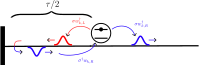
\includegraphics[width = 1 \linewidth]{figures/mirror_feedback.pdf}
    \caption{Illustration of a two-level system coupled to a semi-infinite waveguide, where one end of the waveguide terminates at a mirror reflecting incoming photons. The left propagating mode (red) propagates for a time $\tau/2$ until it gets reflected into the right propagating mode (blue) that returns to the emitter after a total time of $\tau$.}
    \label{fig:feedback_sketch}
\end{figure}

\section{Semi-Infinite Waveguide}
We consider a Semi-Infinite Waveguide terminating with a mirror in one end, as also depicted in Fig.~\ref{fig:feedback_sketch}. The mirror will here introduce a face shift $\phi$, but also an excitation emitted in the left mode will, after a delay time of $\tau/2$, be reflected into the right mode and thus, after a total delay time of $\tau$ hit the emitter again. The left and right propagating modes are, however, symmetrical \cite{ArranzRegidor2021ModelingModel}, and one can instead think of a single mode wrapping around the emitter. The waveguide is thus a "horseshoe", and the emitter couples to two points of the horseshoe. This is also illustrated in Fig.~\ref{fig:horseshoe}. With this mental picture, there is only one propagating mode, and we describe the interaction through the Hamiltonian \cite{Whalen2019CollisionTrajectories}:
\begin{equation}
    H_k = \mathrm{e}^{i \phi} \sqrt{\gamma/2\Delta t} \left( \sigma^\dagger w_{k} + \sigma w_{k}^\dagger \right) + \sqrt{\gamma/2\Delta t} \left( \sigma^\dagger w_{k+\Tilde{\tau}} + \sigma w_{k+\Tilde{\tau}}^\dagger \right) \label{eq:tls_feedback}
\end{equation}
where $\Tilde{\tau} = \tau/\Delta t$ is the index necessary to introduce a time-delay of $\tau$. Note that it is the operator $w_{k+\Tilde{\tau}}$ that never "sees" the emitted photon again (thus corresponding to the left propagating mode in Fig~\ref{fig:feedback_sketch}), whereas the operator $w_{k}$ experiences the emitted photon from $\Tilde{\tau}$ time steps ago (and thus corresponds to the right propagating mode in Fig.~\ref{fig:feedback_sketch}).  $w_{k}^\dagger$ and $w_{k}$ thus carry the phase factor $\mathrm{e}^{i \phi}$ from the mirror. 

\begin{figure}[H]
    \centering
    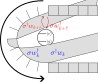
\includegraphics[width=0.5\linewidth]{figures/horseshoe.pdf}
    \caption{Numerical illustration of the semi-infinite waveguide, where the emitter couples to two points of the waveguide such that previous emission re-interacts with the emitter. $\Tilde{\tau} = \tau/\Delta t$ is here the index that induces the time delay $\tau$ between the emission and reabsorption of the emitted pulse. The blue and red interaction carries a phase difference of $\phi$.}
    \label{fig:horseshoe}
\end{figure}

With the Hamiltonian in eq.~\eqref{eq:tls_feedback}, we can simulate how an initially excited emitter decays. In Code Sample \ref{ls:time_delay_code}, we show how to construct the time delayed operator $w_{k+\Tilde{\tau}}$. Notice the simplicity in setting up the simulation. We define two time-delayed operators in the Hamiltonian, and suddenly we can simulate non-Markovian effects. The rest of the code and functions used are the same as previously, allowing for a painless user experience. This modality or separation of features also allows for great customization in the systems that can be studied. The software is thus truly versatile and not just well-defined to solve a restricted set of pre-defined problems.

In Fig.~\ref{fig:tls_feedback}, we plot the population of the emitter as a function of time. We consider two mirror phases $\phi = \pi$ and $\phi = 0$ both $\tau = 1/\gamma$. For reference, we also plot the case of $\tau = \infty$, meaning no memory effects. We see two very distinct population evolutions depending on the phase of the mirror. For $\phi = 0$, the reflected photon interferes constructively with the emission of a photon in the right propagating mode from the emitter.  This leads to a faster decay of the emitter, which is evident by comparing with the case of $\tau=\infty$. Thus, The emitter emits a photon that leads to stimulated emission with itself! With $\phi = \pi$, we instead have destructive interference, and the excitation can never escape to the right. This leads to excitation being trapped, and the system goes to a steady state where the emitter has a constant population of $\approx 0.5$. 




\begin{listing}[H]
\begin{minted}[
frame=lines,
framesep=2mm,
baselinestretch=1.2,
bgcolor=LightGray,
fontsize=\small,
linenos,
escapeinside=||,
mathescape=true
]{julia}
times = 0:0.1:12 #Times for setting up waveguide basis
dt = times[2]-times[1]
be = FockBasis(1)
bw = WaveguideBasis(1,1,times)
sdw = create(be) |$\otimes$| destroy(bw)
wds = destroy(be) |$\otimes$| create(bw)

gamma = 1 #Decay rate of emitter
delay_time = 1 #In units of gamma
phi = pi #Mirror phase

#Creat delayed waveguide operator with delay keyword
sdw_delay = create(be) |$\otimes$| destroy(bw;delay=delay_time/dt)
wds_delay = destroy(be) |$\otimes$| create(bw;delay=delay_time/dt)

H = exp(i*phi)*sqrt(gamma/2/dt)*(sdw+wds)+sqrt(gamma/2/dt)*(sdw_delay+wds_delay)

#Operator for emitter population
sd = create(be) |$\otimes$| identityoperator(bw)
s = destroy(be) |$\otimes$| identityoperator(bw)
n = ad*a
function ne_exp(time,psi)
    expect(n,psi)
end

psi_initial = fockstate(be,1) |$\otimes$| zerophoton(bw) #Initial state
times_sim = 0:0.1:10 #Simulation time has to be smaller than times due to delay. 
tout, ne_pi = waveguide_evolution(times_sim, psi_initial, H,fout=ne_exp)
\end{minted}
\caption{Code for simulating delayed feedback in the waveguide illustrated in Fig.~\ref{fig:horseshoe}. Lines 1-6 set up the standard waveguide basis, emitter basis, and waveguide operators. Lines 8-10 set up the parameters for the simulation. Lines 13-14 set up the delayed waveguide operators $\sigma^\dagger w_{k+\Tilde{\tau}}$ and $\sigma w^\dagger_{k+\Tilde{\tau}}$ by using the keyword \code{delay}. The rest simulates the population of the emitter.}
\label{ls:time_delay_code}
\end{listing}


\begin{figure}[H]
    \centering
    \includegraphics[width = 0.5\linewidth]{figures/tls_mirror_pop.pdf}
    \caption{The population of a two-level system coupled to a semi-infinite waveguide with a mirror in one end. The mirror is located such that a round trip from the emitter to the mirror takes $\tau$ time, and the mirror induces a phase change of $\phi = 0$ and $\phi = \pi$, respectively. This leads to either a faster decay of the emitter or excitation trapping, where the emitter does not decay further. The case where the mirror is placed infinitely far away $\tau = \infty$ is also shown for reference.}
    \label{fig:tls_feedback}
\end{figure}

We can also simulate how an incoming single-photon Gaussian state scatters off on this system. In Fig.~\ref{fig:onephoton_pulse}, we consider an initial Gaussian single photon state: $\ket{\psi}_{in} = \sum_k \xi^{(1)}(t_k) \sqrt{\Delta t} \ket{1_k}$ with $\xi^{(1)}$ defined in eq.~\eqref{eq:gaussian}. The pulse has a width of $\sigma = 0.5 / \gamma$, and the delay from the mirror is still $\tau = 1/\gamma$. For reference, we also show the case of a single-sided cavity ($\tau = 0$) as studied in ch.~\ref{ch2} and \ref{ch3}. In Fig.~\ref{fig:onephoton_pulse}(a), we show the two-level-system population as a function of time. Most noticeably, we do not see an excitation trapping, no matter the phase change of the mirror. A stronger reflection of the pulse when the mirror phase change is $\phi = \pi$ (red) is seen as a much lower excitation probability of the emitter. The first part of the pulse here reflects off the mirror and interferes with the later part of the pulse leading to a strong reflection. This is evident in Fig.~\ref{fig:onephoton_pulse}(b), where we consider the scattered wavefunctions. For $\phi = \pi$, the reflected wavefunction has a Gaussian output shape with a strongly suppressed "tail." For reference, the single-sided scattered wavefunction (black $\tau=0$) shows a distorted shape with two peaks. For $\phi = 0$, the single-photon output state is even more distorted, with an extra peak arising, most likely due to multiple interactions with the emitter.  


\begin{figure}[H]
    \centering
    \includegraphics[width=\linewidth]{figures/pulse_wf.pdf}
    \caption{(a) Same as Fig~\ref{fig:tls_feedback}, but with an incoming Gaussian single-photon state with width $\sigma = 0.5 /\gamma$. (b) The scattered wavefunction after the incoming Gaussian pulse has interacted with the emitter and mirror. }
    \label{fig:onephoton_pulse}
\end{figure}

Finally, we can instead consider a two-photon Gaussian pulse on the semi-infinite waveguide with a mirror. In Fig~\ref{fig:twophoton_mirror}(a), we show the two-photon scattered wavefunction for a two-photon Gaussian product state $\ket{\psi}_{in} = \sum_k \sum_j \xi^{(1)}(t_k)\xi^{(1)}(t_j) \Delta t w_k^\dagger w_j^\dagger \ket{\emptyset}$ with the same parameters as the single-photon state. In Fig.~\ref{fig:twophoton_mirror}(b), the SVD of the scattered state is also shown. For $\phi = \pi$, we observe excitation trapping, which is evident from $\sum_i \lambda_i^2 \neq 1$ in the SVD. We also see that the scattered wavefunction is in a product state since only one important SVD mode is occupied. This starkly contrasts with what is observed for $\phi = 0$, where the scattered wavefunction occupies two modes almost equally with $\lambda_1^2 \approx \lambda_2^2 \approx 0.5$. We furthermore see that the wavefunction for $\phi=0$ shows almost no occupation along the diagonal, meaning that observing two photons simultaneously is not very likely. Compared with the single-sided case $\tau=0$, this is very different since spontaneous emission here leads to a very pronounced diagonal. This again shows that the two photons for $\phi=0$ are separated in time after the interaction.  

\

In refs. \cite{Witthaut2012PhotonEmitters,Lund2023PerfectPulse} the authors propose schemes for sorting and distinguishing between single-photon and two-photon pulses. Based on the very limited study above, it is possible to imagine that similar schemes can be devised and perhaps even improved if considering a waveguide system with feedback. Indeed, in ref. \cite{Nemet2019StabilizingTemperature}, they show that time-delayed feedback from a bosonic phonon bath can help stabilize the coherence of an emitter in an optical cavity. Similarly, it is interesting to consider whether there exists any scheme that can take advantage of non-markovian dynamics in waveguide QED systems. In ref. \cite{Pichler2017UniversalFeedback} a scheme to generate 2D photonic cluster states using feedback in a waveguide is, for example, proposed. Although simulating such 2D photonic cluster states might require the introduction of matrix product states, it is possible that similar schemes involving fewer photons might be analyzed or devised with the help of the numerical framework. Such investigations are a natural extension of the study shown here and an obvious use case for the numerical framework presented. 


\begin{figure}
    \centering
    \includegraphics[width=\linewidth]{figures/twophoton_mirror.pdf}
    \caption{(a): The scattered two-photon Gaussian pulse for the same configuration and parameters  considered in Fig.~\ref{fig:tls_feedback} and \ref{fig:onephoton_pulse}. In the first row, the mirror phase is $\phi = \pi$, in the second row, it is $\phi=0$, and in the last row, we consider no delay $\tau=0$ (single-sided). All contour plots have been normalized so that the largest value is unity. (b): The SVD of the two-photon scattered state in (a). For $\phi=\pi$, we observe excitation trapping and thus $\sum_i \lambda_i^2 \neq 1$.}
    \label{fig:twophoton_mirror}
\end{figure}